%%%%%%%%%%%%%%%%%%%%%%%%%%%%%%%%%%%%%%%%%%%%%%%%%%%%%%%%%%%%%%%%%
% MUW Presentation
% LaTeX Template
% Version 1.0 (27/12/2016)
%
% License:
% CC BY-NC-SA 4.0 (http://creativecommons.org/licenses/by-nc-sa/3.0/)
%
% Created by:
% Nicolas Ballarini, CeMSIIS, Medical University of Vienna
% nicoballarini@gmail.com
% http://statistics.msi.meduniwien.ac.at/
%
% Customized for UAH by:
% David F. Barrero, Departamento de Automática, UAH
%%%%%%%%%%%%%%%%%%%%%%%%%%%%%%%%%%%%%%%%%%%%%%%%%%%%%%%%%%%%%%%%%

\documentclass[10pt,compress]{beamer} % Change 10pt to make fonts of a different size
\mode<presentation>

\usepackage[spanish]{babel}
\usepackage{fontspec}
\usepackage{tikz}
\usepackage{etoolbox}
\usepackage{xcolor}
\usepackage{xstring}
\usepackage{listings}

% Custom packages
\usepackage{standalone}
\usepackage{multicol}
\usepackage{multirow} % Confusion matrix
\usepackage{tikz}
\usepackage{pgfplots}
\def\layersep{2.5cm}
\usetikzlibrary{matrix,chains,positioning,decorations.pathreplacing,arrows,shapes}

\definecolor{dkgreen}{rgb}{0,0.6,0}
\definecolor{gray}{rgb}{0.5,0.5,0.5}
\definecolor{mauve}{rgb}{0.58,0,0.82}
 

\usetheme{UAH}
\usecolortheme{UAH}
\setbeamertemplate{navigation symbols}{} 
\setbeamertemplate{caption}[numbered]

%%%%%%%%%%%%%%%%%%%%%%%%%%%%%%%%%%%%%%%%%%%%%%%%%%%%%%%%%%%%%%%%%
%% Presentation Info
\title[Supervised learning]{Supervised learning}
\author{\asignatura\\\carrera}
\institute{}
\date{Departamento de Automática}
%%%%%%%%%%%%%%%%%%%%%%%%%%%%%%%%%%%%%%%%%%%%%%%%%%%%%%%%%%%%%%%%%


%%%%%%%%%%%%%%%%%%%%%%%%%%%%%%%%%%%%%%%%%%%%%%%%%%%%%%%%%%%%%%%%%
%% Descomentar para habilitar barra de navegación superior
\setNavigation
%%%%%%%%%%%%%%%%%%%%%%%%%%%%%%%%%%%%%%%%%%%%%%%%%%%%%%%%%%%%%%%%%

%%%%%%%%%%%%%%%%%%%%%%%%%%%%%%%%%%%%%%%%%%%%%%%%%%%%%%%%%%%%%%%%%
%% Configuración de logotipos en portada
%% Opacidad de los logotipos
\newcommand{\opacidad}{1}
%% Descomentar para habilitar logotipo en pié de página de portada
\renewcommand{\logoUno}{Images/isg.png}
%% Descomentar para habilitar logotipo en pié de página de portada
%\renewcommand{\logoDos}{Images/CCLogo.png}
%% Descomentar para habilitar logotipo en pié de página de portada
%\renewcommand{\logoTres}{Images/ALogo.png}
%% Descomentar para habilitar logotipo en pié de página de portada
%\renewcommand{\logoCuatro}{Images/ELogo.png}
%%%%%%%%%%%%%%%%%%%%%%%%%%%%%%%%%%%%%%%%%%%%%%%%%%%%%%%%%%%%%%%%%

%%%%%%%%%%%%%%%%%%%%%%%%%%%%%%%%%%%%%%%%%%%%%%%%%%%%%%%%%%%%%%%%%
%% FOOTLINE
%% Comment/Uncomment the following blocks to modify the footline
%% content in the body slides. 


%% Option A: Title and institute
\footlineA
%% Option B: Author and institute
%\footlineB
%% Option C: Title, Author and institute
%\footlineC
%%%%%%%%%%%%%%%%%%%%%%%%%%%%%%%%%%%%%%%%%%%%%%%%%%%%%%%%%%%%%%%%%


\begin{document}

%%%%%%%%%%%%%%%%%%%%%%%%%%%%%%%%%%%%%%%%%%%%%%%%%%%%%%%%%%%%%%%%%
% Use this block for a blue title slide with modified footline
{\titlepageBlue
    \begin{frame}
        \titlepage
    \end{frame}
}

\institute{\asignatura}

\begin{frame}[plain]{}
   \begin{block}{Objectives}
      \begin{enumerate}
         \item Define Machine Learning (ML)
		 \item Delimite ML scope
         \item Introduce the main ML tasks
         \item Recognize problems as ML tasks
      \end{enumerate} 
   \end{block}

   \begin{block}{Bibliography}
	\begin{itemize}
        \item Bishop, Christopher M. \textit{Pattern Recognition and Machine Learning}. 2nd edition. Springer-Verlag. 2011
        \item M\"uller, Andreas C., Guido, Sarah. \textit{Introduction to Machine Learning with Python}. O'Reilly. 2016
	\end{itemize}
   \end{block}
\end{frame}

{
\disableNavigation{white}
\begin{frame}[shrink]{Table of Contents}

 	\frametitle{Table of Contents}
  	\begin{multicols}{2}
  		\tableofcontents
    \end{multicols}

 %\frametitle{Table of Contents}
 %\tableofcontents
  % You might wish to add the option [pausesections]
\end{frame}
}

\subsection{Linear regression}

\begin{frame}{Algorithms}{Linear regression (I)}
     Lineal regression assumes a linear relationship among variables
	\begin{itemize}
		\item This limitation can be easely overcome
		\item Surprisingly good results in high dimensional spaces
	\end{itemize}

    \begin{columns}
 	   \column{.60\textwidth}
        \begin{block}{Lineal regression}
            $y = a_0 + a_1 x_1  + a_2 x_2 + \dots + a_n x_n$
        \end{block}

 	   \column{.40\textwidth}
		\begin{figure}
	        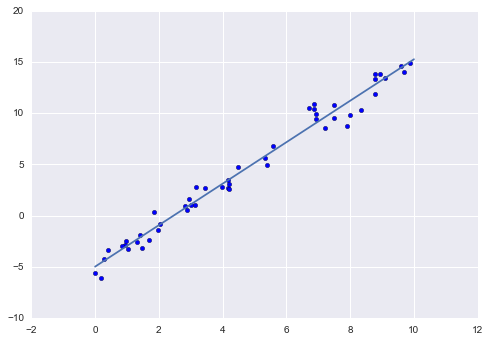
\includegraphics[width=\textwidth]{figs/regression.png}
		\end{figure}
    \end{columns}

\end{frame}

%\begin{frame}{Linear regression (II)}
%    Example: Does money make people happier? (example from (G\'eron, 2017))
%    \bigskip

%    \begin{columns}
%       \column{.40\textwidth}
%        \begin{tabular}{ccc}\hline
%            \texttt{Country} & \texttt{GDP} & \texttt{\textit{LS}} \\\hline
%            Hungary& 12,240  & \textit{4.9}   \\
%            Korea   & 27,195  & \textit{5.8}   \\
%            France & 37,675  & \textit{6.5}   \\
%            Australia & 50,962 & \textit{7.3} \\
%            USA     & 55,805  & \textit{7.2}   \\
%            \hline
%        \end{tabular}\\
%        LS =Life satisfaction

%       \column{.60\textwidth}
%            \begin{exampleblock}{Linear regression}
%                \centering \includegraphics[width=0.9\linewidth]{Images/scattergdpregression.png}
%                \vspace{-0.4cm}
%                \begin{equation*}
%                life\_satisfaction = \theta_0 + \theta_1 \times GDP\_per\_capita
%                \end{equation*}
%                \vspace{-0.2cm}
%            \end{exampleblock}
%    \end{columns}
%\end{frame}

\begin{frame}{Algorithms}{Linear regression (II)}
	Several methods to fit coefficients
	\begin{itemize}
		\item Ordinary Least Squares (OLS)
        \item Generalized Least Squares (GSL)
        \item Weighted Least Squares (WLS)
		\item Generalized Least Squares with AR Covariance Structure (GLSAR)
	\end{itemize}

	\alert{Regularization}: Term that penalizes complexity
	\begin{itemize}
		\item L1 (Lasso regression) 
		\item L2 (Ridge regression)
		\item ElasticNet: L1 and L2
	\end{itemize}

    \begin{columns}
 	   \column{.3\textwidth}
    		\begin{block}{Lasso}
            	$\lambda \sum_j^n \beta_j^2$
        	\end{block}

	   \column{.3\textwidth}
     		\begin{block}{Ridge}
            	$\lambda \sum_j^n |\beta_j|$
        	\end{block}
	   \column{.4\textwidth}
     		\begin{block}{ElasticNet}
			$\alpha  \sum_j^n \beta_j^2 + (1-\alpha) \sum_j^n |\beta_j|$
        	\end{block}
    \end{columns}

\end{frame}

\subsection{ARIMA}
\begin{frame}{Algorithms}{ARIMA (I)}
    \begin{columns}
 	   \column{.5\textwidth}
	   AR: Autoregressive model
	    \begin{itemize}
		\item Current observation depends on the last $p$ observations
		\item Long term memory
	    \end{itemize}

	   \column{.5\textwidth}
		\begin{block}{AR(p)}
			$X_t = c+\sum_{i=1}^p \phi_i X_{t-1}+\epsilon_t$
        	\end{block}
    \end{columns}

    \smallskip

    \begin{columns}
 	   \column{.5\textwidth}
	   MA: Moving Average model
	    \begin{itemize}
		\item Current observation linearly depends on the last $q$ innovations
		\item Short term memory
	    \end{itemize}

	   \column{.5\textwidth}
		\begin{block}{MA(q)}
			$X_t =  \mu + \epsilon_t + \theta_1 \epsilon_{t-1} + ... + \theta_q \epsilon_{t-q}$
        	\end{block}
    \end{columns}

    \bigskip

    ARMA model = AR + MA
	\begin{itemize}
		\item ARMA(p, q): Two hyperparameters, p and q
	\end{itemize}

\end{frame}

\begin{frame}{Algorithms}{ARIMA (II)}
	ARIMA = AR + i + MA (AR integrated MA)
    \begin{itemize}
	\item ARIMA(p, d, q)
	\item Three integer parameters: p, q and d (in practice, low order models)
    \end{itemize}

    \centering 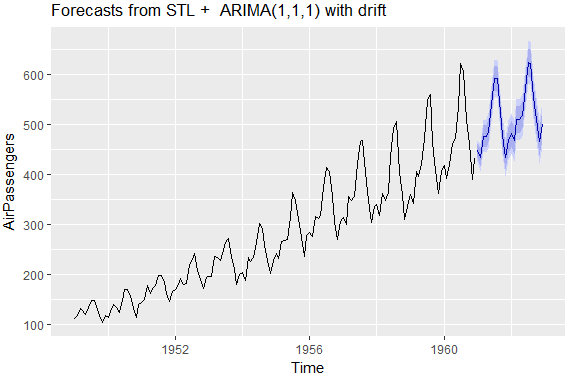
\includegraphics[width=0.6\linewidth]{figs/arima.png}

    \tiny{\href{https://itnext.io/understanding-the-forecasting-algorithm-stlf-model-29d74b3a0336?gi=282b647b24a7}{(Source)}}

    \normalsize
	\flushleft
    \alert{autoarima}: search over p, q and d
\end{frame}



\end{document}
